%----------------------------------------------------------------------------------------
%	PACKAGES AND OTHER DOCUMENT CONFIGURATIONS
%----------------------------------------------------------------------------------------

\documentclass[12pt]{article} % Default font size is 12pt, it can be changed here

\usepackage{geometry} % Required to change the page size to A4
\geometry{a4paper} % Set the page size to be A4 as opposed to the default US Letter

\usepackage{graphicx} % Required for including pictures

\usepackage{float} % Allows putting an [H] in \begin{figure} to specify the exact location of the figure
\usepackage{wrapfig} % Allows in-line images such as the example fish picture
\usepackage{psfrag,amsmath,amsfonts,amsthm,amssymb,cite}
\usepackage{lipsum} % Used for inserting dummy 'Lorem ipsum' text into the template

\linespread{1.2} % Line spacing

%\setlength\parindent{0pt} % Uncomment to remove all indentation from paragraphs

\graphicspath{{Pictures/}} % Specifies the directory where pictures are stored

\begin{document}

%----------------------------------------------------------------------------------------
%	TITLE PAGE
%----------------------------------------------------------------------------------------

\begin{titlepage}

\newcommand{\HRule}{\rule{\linewidth}{0.5mm}} % Defines a new command for the horizontal lines, change thickness here

\center % Center everything on the page

\textsc{\LARGE CS4516: Empirical Results}\\[1.5cm] % Name of your university/college

\HRule \\[0.4cm]
{ \huge \bfseries Tag-Based IP Spoofing Prevention Under Low Deployment Scenarios}\\[0.4cm] % Title of your document
\HRule \\[1.5cm]

\begin{minipage}{0.4\textwidth}
\begin{flushleft} \large
\emph{Author:}\\
Michael Calder\\
Daniel Robertson\\
\end{flushleft}
\end{minipage}
~
\begin{minipage}{0.4\textwidth}
\begin{flushright} \large
\emph{Supervisor:} \\
Dr. Craig Shue % Supervisor's Name
\end{flushright}
\end{minipage}\\[4cm]

{\large \today}\\[3cm] % Date, change the \today to a set date if you want to be precise

%\includegraphics{Logo}\\[1cm] % Include a department/university logo - this will require the graphicx package

\vfill % Fill the rest of the page with whitespace

\end{titlepage}

%----------------------------------------------------------------------------------------
%	TABLE OF CONTENTS
%----------------------------------------------------------------------------------------

%\tableofcontents % Include a table of contents

\newpage % Begins the essay on a new page instead of on the same page as the table of contents 


%----------------------------------------------------------------------------------------
% -- Paper Outline --
%----------------------------------------------------------------------------------------

\section{Results and evaluation of our two approaches}

After implementing the hash-chain and TOTP-inspired protocols using NS-3, analysis of the results has shown that both methods offer significant security benefits without causing problems with performance. Each of the two approaches has its own advantages; in this section we will examine these differences and explain how each of the hash functions affect security and performance.

The time interval we used for both methods was about half a minute (32 seconds) but could easily be adjusted to add security or space-efficiency. We chose this time interval because we were never able to crack any collisions in less than half a minute when attempting to brute force a hash. With the hash-chain approach, a compromised hash can only be exploited within the duration of the time interval it was created with. Also, no matter how many hashes we captured, we were not able to determine the original tag (mostly due to collisions) which prevents an attacker from determining future hashes. The only downside of this approach is space complexity. If the interval is roughly half a minute and one day of hashes are generated at a time, 2880 hashes (11KB for xxHash, 46KB for SHA-1) must be stored in RAM. These amounts are not beyond the capabilities of popular routers, but obviously requiring one fourth the space is preferable. Note that as the time interval gets smaller, these numbers grow significantly. Using a 128-bit hash like SHA-1 will also use up four times as much memory as a 32-bit hash like xxHash. With that said, these issues can be negated increasing how often the hashes are generated (i.e. twice a day).

For the TOTP-inspired approach, each compromised hash also proved useful for a maximum of 32 seconds and then became useless. Because the original tag cannot easily be determined due to collisions (even if the method for combining the timestamp with the tag is known), this method also made stolen hashes unhelpful to attackers in predicting future hashes. Almost no additional memory is needed for this approach and the time interval can be adjusted as desired. The downside to this approach is that, with a lot of work, the original tag can be determined. Using rainbow tables, knowledge of how the timestamp is combined with the tag, and a lot of CPU, having multiple compromised hashes and timestamps can allow an attacker to determine the original tag by comparing the brute-force results until there is only one common tag in the lists of collisions. With that said, breaking this system now becomes very difficult and time-intensive to acquire only one tag.

\begin{figure}[ht!]
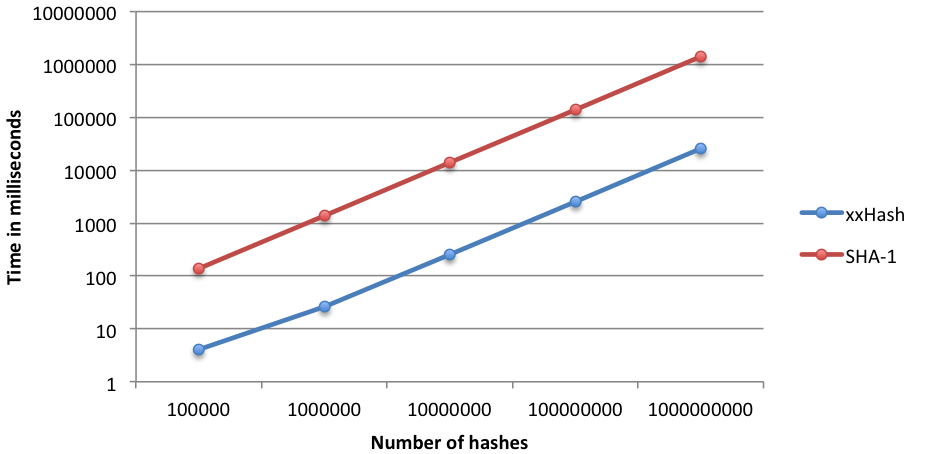
\includegraphics[width=160mm]{hashspeeds.png}
\caption{Hash speeds for xxHash and SHA-1 on a 2.4GHz processor}
\end{figure}

The main differences between cryptographic and non-cryptographic hash functions seemed to be the speed. xxHash, being the fastest non-cryptographic hash algorithm, ran up to 40 million hashes per second. SHA-1, being one of the fastest cryptographic hash algorithms, maxed out around 728 thousand hashes per second. In practice, xxHash caused no measurable latency in the test network (same speeds to the millisecond) while SHA-1 failed to meet this requirement. For the once-a-day calculations required for hash chaining, the speeds (on a 2.4GHz processor, which was used to simulate the network) are shown in Figure 1. As far as security is concerned, rainbow tables render both algorithms just as difficult to brute-force. When the original tag is 48 bits, almost 300 trillion possibilities need to be iterated through before a list of all possible original tags that could produce a given hash is known.

So why not use xxHash in any context? xxHash is not a cryptographic hashing algorithm because it is not second preimage resistant, which means that it is possible to determine potential collisions without using brute-force methods. This can be insecure in some contexts, but for what we are trying to accomplish it does not cause an issue because collisions cannot be leveraged. If anything, more collisions only complicate the process of attempting to reverse each hash in a hash chain or trying to determine the original tag from a TOTP-inspired hash. For the purposes of making compromised tag-hashes not a security concern, we have concluded that both of our approaches (using xxHash) are effective and have the potential to provide any reasonable desired space and time efficiency.




%----------------------------------------------------------------------------------------
%	BIBLIOGRAPHY
%----------------------------------------------------------------------------------------

%\bibliography{references.bib}

%----------------------------------------------------------------------------------------

\end{document}
